\documentclass[a4paper,12pt]{report}
\usepackage[T2A]{fontenc}
\usepackage[russian]{babel}
\usepackage{subcaption}
\usepackage{amsmath}
\usepackage{amssymb}
\usepackage{amsthm}
\usepackage{float} 
\usepackage{lscape}
\usepackage{array}
\usepackage[matrix,arrow,curve]{xy}
\usepackage{graphicx}
\usepackage{makecell}
\usepackage{titlesec}
\usepackage{titletoc}
\usepackage{blkarray}
\usepackage{rotating}
\usepackage{longtable}
\usepackage{geometry}
\usepackage{fancyhdr}
\usepackage{enumitem}
\newlist{steps}{enumerate}{1}
\setlist[steps, 1]{label = Step \arabic*:}
\usepackage{diagbox} 
\usepackage{multirow}
\usepackage{url}
\usepackage{listings}
\lstset
{
    language=C++, % выберите язык программирования
    basicstyle=\ttfamily, % шрифт для кода
    keywordstyle=\color{blue}, % стиль ключевых слов
    commentstyle=\color{green!60!black}, % стиль комментариев
    stringstyle=\color{red}, % стиль строк
    showstringspaces=false, % не показывать пробелы в строках
    frame=single, % рамка вокруг кода
    numbers=left, % номера строк
    numberstyle=\tiny, % стиль номеров строк
    breaklines=true % перенос строк, если необходимо
}
\usepackage{tabularx}

%\usepackage{hyperref}

% \textwidth=175mm  \textheight=257mm
% \voffset=-2.64cm  \hoffset=-1.85cm
\geometry{tmargin=2cm,bmargin=2cm,lmargin=2.5cm,rmargin=1cm}

\fancyhf{}
\renewcommand{\headrulewidth}{0pt}
\fancyhead[C]{\thepage}
\pagestyle{fancy}
\fancypagestyle{plain}{%
  \fancyhf{} % clear all header and footer fields
  \renewcommand{\headrulewidth}{0pt}
  \fancyhead[C]{\thepage} % except the center
}
\setlength{\headheight}{20pt}

\renewcommand{\thesection}{\arabic{chapter}.\arabic{section*}}
\renewcommand{\thesubsection}{\arabic{chapter}.\arabic{section*}.\arabic{subsection}}

\usepackage{xcolor,paracol}
\setlength{\parindent}{15pt}

\setcounter{page}{1} 
\renewcommand{\baselinestretch}{1.2}
\newtheorem{acknowledgement}{Благодарность}

\newtheorem{definition}{Определение}[chapter]
\newtheorem{lemma}{Lemma}[chapter]
\newtheorem{theorem}{Theorem}[chapter]
\newtheorem{remark}{Замечание}[chapter]
\newtheorem{proposition}{Утверждение}[chapter]
\newtheorem{property}{chapter}
\newtheorem{corollary}{Следствие}[chapter]
\newtheorem{assumption}{Assumption}[chapter]
\newtheorem{example}{Пример}[chapter]

\renewcommand{\thesection}{\arabic{chapter}.\arabic{section*}}
\renewcommand{\theequation}{\arabic{chapter}.\arabic{equation}}
\newcommand{\secref}[1]{\S\ref{#1}}
\renewcommand*\footnoterule{}

\usepackage{color}
\definecolor{HREF-COLOR}{RGB}{10,54,100}
\usepackage[unicode, colorlinks, urlcolor=HREF-COLOR, linkcolor=Violet, pagecolor=Violet]{hyperref}

\pagecolor{white}
\author{\href{https://github.com/ypodlesov}{Егор Подлесов}}
\title{\textbf{Численное решение одномерного уравнения Лапласа на отрезке}}

\begin{document}

    \maketitle
    \clearpage

    \section*{Описание исходной задачи}

    Необходимо решить краевую задачу Дирихле для уравнения Лапласа
    
    \begin{equation*}
     \begin{cases}
       -u'' = f\\
       u(0) = a, u(1) = b 
     \end{cases}
    \end{equation*}
    численно с помощью метода конечных разностей.
    \newline
    Решаем задачу на интервале $(0, 1)$, вводя на ней равномерную сетку $x_0, x_1, ..., x_N$,
    $x_i = i * h$,
    $h = \frac{1}{N}$
    Дискретная аппроксимация уравнения:
    $$-\frac{y_{i-1}-2y_i+y_{i+1}}{h^{2}} = f(x_i)$$
    
    для приграничных узлов $(x_1, x_{N-1})$
    сюда войдут граничные условия
    
    \section*{Метод прогонки}
    
    $a_i$ - элементы стоящие на поддиагонали в $i$-ой строке
    \newline
    $b_i$ - элементы стоящие на диагонали в $i$-ой строке
    \newline
    $c_i$ - элементы стоящие на наддиагонали в $i$-ой строке
    \newline
    $d_i$ - элемент правой части в $i$-ой строке
    \newline
    
    Прямая прогонка состоит в вычислении прогоночных коэффициентов $\alpha_i$ и $\beta_i$ , где $i$ – номер строки матрицы. Этот этап выполняется при $i = 1...n$ строго по возрастанию значения $i$.

    \begin{enumerate}
        \item В первой строке матрицы $i = 1$ используются формулы:
    \[\mathbf{y_1=b_1, \alpha_1=\frac{-c_1}{y_1}, \beta_1=\frac{d_1}{y_1}}\]
        \item Для строк $i$ от $2$ до $N-2$ используются рекуррентные формулы:
    \[\mathbf{y_i=b_i+a_i*\alpha_{i-1}, \alpha_i=\frac{-c_i}{y_i}, \beta_i=\frac{(d_i-a_i*\beta_{i-1})}{y_i}}\]
        \item При $i = N - 1$ прямая прогонка завершается вычислением: 
    \[\mathbf{y_{N-1}=b_{N-1}+a_{N-1}*\alpha_{N-2}, \beta_{N-1}=\frac{(d_{N-1}-a_{N-1}*\beta_{N-2})}{y_{N-1}}}\]
    
    После этого производится обратная прогонка, в которой происходит вычисление неизвестных $yi$. Этот этап выполняется при $i = n...1$ строго по
    убыванию значения $i$.
        \item В последней строке матрицы $i = N - 1$ выполнено $x_{N-1} = \beta_{N-1}$
    \newline
        \item Для всех остальных строк при $i$ от $N-2$ до $1$ применяется формула:
    \[\mathbf{x_i=\alpha_i*x_{i+1}+\beta_{i}}\]

    \end{enumerate}

    \section*{График}
    
    График зависимости точности с-нормы и дискретной l2-нормы от шага сетки в логарифмическом виде

    
    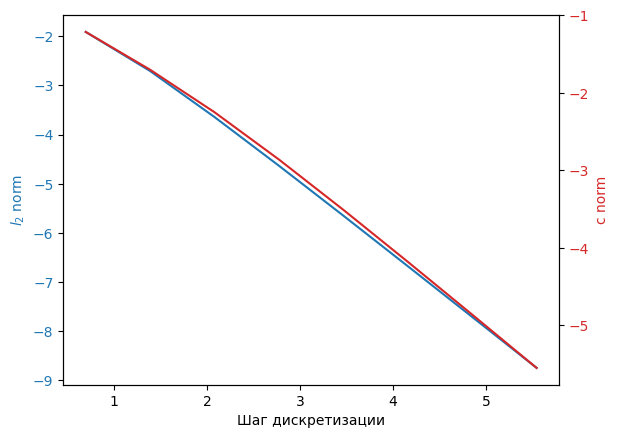
\includegraphics[width=0.99\linewidth]{graph.jpeg}
    

    

\end{document}
